\documentclass{bmvc2k}

%% Enter your paper number here for the review copy
\bmvcreviewcopy{243}

\title{When AI-Image Detectors Learn the Benchmark\\ Instead of the Generator}

% Anonymous authors for double-blind review.
% \bmvcreviewcopy replaces the author block automatically.
\addauthor{Anonymous}{}{1}

\addinstitution{
 Anonymous Institution
}

\runninghead{Anonymous}{Eigenfraud: Auditing AI-Image Detectors}

% Macros (do not begin with \bmva, to avoid clashing with the class file).
\def\eg{\emph{e.g}\bmvaOneDot}
\def\Eg{\emph{E.g}\bmvaOneDot}
\def\etal{\emph{et al}\bmvaOneDot}

% Additional packages used for tables.
\usepackage{booktabs}
\usepackage{amsmath}
\usepackage{amssymb}

%-------------------------------------------------------------------------
\begin{document}

\maketitle

\begin{abstract}
Synthetic image detectors report near-perfect benchmark scores but fail when applied outside their training conditions. Prior work attributes this to distribution shift in generative models, but we demonstrate that a simpler explanation accounts for the majority of reported benchmark success: popular benchmarks encode the real-versus-fake label in file format and resolution, and detectors learn the shortcut \emph{exclusively}, with no residual generative signal. We propose evaluating detectors across benchmarks that vary in shortcut severity, and introduce format normalization as a control to separate metadata shortcuts from pixel-level ones.

We test six public detectors on CIFAKE (no format or resolution bias), Defactify (resolution bias only), and GenImage (severe format and resolution bias). On CIFAKE, all six detectors score below chance, with several calling real images fake more often than fakes. On GenImage, which shares the JPEG$=$real, PNG$=$fake pattern from their training data, AUC jumps by an average of $0.53$ across five detectors --- a regime change, not a robustness fluctuation. Re-encoding every image to $256\times256$ PNG does not recover CIFAKE performance, confirming the shortcut is embedded in pixel statistics and cannot be removed by format normalization alone. One detector, B-Free, behaves differently: its DINOv2 features rise from $0.497$ to $0.637$ on CIFAKE, indicating it responds to visual quality differences that frequency-heavy models do not exploit. Below-chance performance on an artifact-free benchmark is a clean diagnostic for shortcut-dependent detectors.

To probe causality, we conduct a format-swap experiment: re-encoding real images as PNG and fake images as JPEG reverses the format association. FreqNet collapses to chance and NPR inverts below chance, demonstrating that format is not merely helpful to these detectors --- it is their entire signal on GenImage. Frequency band ablation further localises the shortcut: zeroing the low-frequency band ($r < 0.2\,r_{\max}$) degrades all six detectors substantially on the biased benchmark, with NPR falling by $0.56$ AUC and UnivFD by $0.40$.
\end{abstract}

%-------------------------------------------------------------------------
\section{Introduction}
\label{sec:intro}

AI-image detectors often report strong benchmark performance~\cite{wang2020cnn,corvi2023intriguing,ricker2024aeroblade}, but those numbers are difficult to interpret when the benchmark itself leaks the label. If real and fake images differ in file format, compression history, or canonical resolution, then a detector \emph{will} score well without learning anything about image synthesis, provided the benchmark encodes the label in format. In that case the model is not detecting generation; it is learning the benchmark.

This paper audits that failure mode directly. We study three datasets with very different levels of construction bias:
\begin{enumerate}
  \item \textbf{CIFAKE} is close to an artifact-controlled stress test: both classes are $32\times32$ JPEG.
  \item \textbf{Defactify} removes format bias but retains strong resolution bias.
  \item \textbf{GenImage} contains both severe format and resolution bias.
\end{enumerate}
These artifacts matter because they create shortcuts in exactly the frequency ranges many detectors inspect. A detector can therefore optimise benchmark AUC by exploiting a spurious cue that is easier to learn than generator-specific evidence. We use ``reward hacking'' in that limited sense: a model maximises the benchmark objective by locking onto dataset construction signals rather than the intended concept.

\paragraph{What we show.}
Our results support three concrete claims.
\begin{enumerate}
  \item \textbf{The benchmark bias is measurable.} The ordering of high-frequency divergence is not subtle: CIFAKE $\ll$ Defactify $<$ GenImage.
  \item \textbf{AUC $< 0.5$ is diagnostic, not just bad luck.} On CIFAKE, six external detectors score below chance. This means their decisions are often inverted, which is evidence that they learned a wrong but internally consistent rule.
  \item \textbf{Detector success tracks shortcut availability.} The same detectors that invert on CIFAKE recover very high AUC on GenImage, where the JPEG/PNG shortcut is present again.
\end{enumerate}

\paragraph{Scope and framing.}
This is an audit paper, not a new detector paper. We do not claim to solve AI-image detection. We use public checkpoints, dataset audits, spectral summaries, and controlled re-encoding to ask a narrower question: when a detector performs well, is it recognising generation or exploiting the benchmark?

We additionally conduct two causal experiments not present in the original audit. A \emph{format-swap} experiment reverses the format association (real $\to$ PNG, fake $\to$ JPEG) to test whether format is the mechanism or merely a correlate. \emph{Frequency band ablation} zeroes out low, mid, and high radial bands before evaluation to localise which spectral region carries the shortcut. These experiments support two further claims:
\begin{enumerate}
  \setcounter{enumi}{3}
  \item \textbf{Format is the mechanism, not a correlate.} Reversing the format association collapses FreqNet from $0.977$ to $0.503$ and inverts NPR to $0.381$.
  \item \textbf{The shortcut lives in low frequencies.} Band ablation shows that removing the low-frequency band ($r < 0.2\,r_{\max}$) produces the largest AUC drops, localising the format artifact to the spectral region where JPEG blocking and energy differences manifest.
\end{enumerate}

%-------------------------------------------------------------------------
\section{Related Work}
\label{sec:related}

\paragraph{Frequency cues in synthetic image detection.}
Frequency-domain analyses have long been used to explain why generated images can be separable from photographs~\cite{corvi2023intriguing,frank2020leveraging,durall2020watch}. CNNDetection~\cite{wang2020cnn} popularised the idea that synthetic images share common low-level traces across generators, while later work studied diffusion-era artifacts~\cite{ricker2024aeroblade,synthbuster2023}. Our paper does not dispute that synthetic images may leave traces. It demonstrates that benchmark wins \emph{are} explained by a simpler cue, and identifies the precise spectral locus of that cue.

\paragraph{Shortcut learning and biased benchmarks.}
Grommelt \etal~\cite{grommelt2024} showed that generated-image benchmarks can be strongly confounded by JPEG-related bias. Wang \etal~\cite{wang2023frequency} framed shortcut learning in image classification more broadly, showing that neural networks often exploit frequency cues that correlate with labels but not with semantics. We build on these perspectives by treating AI-image detection as a shortcut-audit problem: if benchmark construction artifacts induce separable spectra, detectors may optimise those artifacts instead of learning generation.

\paragraph{Detectors we audit.}
We evaluate CNNDetection~\cite{wang2020cnn}, FreqNet~\cite{freqnet}, NPR~\cite{npr}, UnivFD~\cite{univfd}, FatFormer~\cite{fatformer}, and B-Free~\cite{bfree}, plus a simple spectral CNN trained in-house. The detector set intentionally mixes frequency-heavy models and foundation-model-based approaches. This lets us ask whether the shortcut problem is confined to one architectural family. The answer is no: inversion on artifact-controlled data appears across the entire evaluated set, with a single partial exception, while only B-Free consistently benefits from removing some confounds.

%-------------------------------------------------------------------------
\section{Methodology}
\label{sec:method}

\subsection{Audit Protocol}
\label{sec:audit_method}

For each dataset split, we record image count, storage format, resolution statistics, and file size. We treat two properties as likely shortcut sources:
\begin{itemize}
  \item \textbf{Format bias:} one class is predominantly JPEG and the other PNG.
  \item \textbf{Resolution bias:} one class occupies a narrow set of canonical sizes while the other spans many natural image sizes.
\end{itemize}

\subsection{Spectral Characterisation}
\label{sec:spectral_method}

To quantify how much these construction choices separate the classes, we compute mean radial log-power spectra for real and fake images. Each image is converted to grayscale, transformed with a 2D FFT, and reduced to a 1D radial profile by azimuthal averaging~\cite{durall2020watch}. For each dataset we report a high-frequency divergence score,
\begin{equation}
\mathrm{HF\text{-}L2} \;=\; \left\lVert \bar{S}_{\mathrm{real}}(r) - \bar{S}_{\mathrm{fake}}(r) \right\rVert_2 \quad \text{for } r > 0.8\,r_{\max},
\label{eq:hfl2}
\end{equation}
where $r_{\max}$ is the Nyquist radius. Equation~\eqref{eq:hfl2} is not meant to be a detector. It is a diagnostic for how strongly dataset construction separates the two classes before any model sees them. Across our three datasets, HF-L2 predicts detector AUC ordering exactly, confirming its value as a pre-evaluation audit metric.

\subsection{Detector Evaluation}
\label{sec:eval_method}

We evaluate six public detectors and one simple spectral CNN using their released checkpoints or the project's saved weights. Our core diagnostic is not only \emph{whether} AUC is high or low, but \emph{how} it fails.

\paragraph{Why below-chance AUC matters.}
If a detector lands near $0.5$ AUC on a new dataset, that may reflect ordinary out-of-distribution failure. If it lands well below $0.5$, then it is usually applying a decision rule in the wrong direction. AUC well below $0.5$ is not a generalisation failure --- it is proof of an internally consistent but inverted decision rule, only diagnosable on an artifact-free benchmark.

\subsection{Normalization as a Diagnostic}
\label{sec:normalize}

To probe whether performance depends on file-format and size mismatches, we also evaluate a normalised variant of the test data. Every image is:
\begin{enumerate}
  \item Converted to RGB (strip alpha channel and EXIF metadata).
  \item Resized to $256 \times 256$ pixels using bilinear interpolation.
  \item Saved as PNG (lossless; no re-JPEG-compression).
\end{enumerate}
This transform is applied identically to both classes. It does not remove content-baked artifacts already present in the pixels, but it does remove trivial differences in container format and nominal resolution. We therefore use normalisation as a diagnostic, not as a claim that all confounds are solved.

\subsection{Format-Swap as a Causal Probe}
\label{sec:swap_method}

Normalisation removes format differences but does not reverse them. To establish a causal link, we conduct a \emph{format-swap} experiment: every real image is re-encoded as PNG (losslessly from JPEG) and every fake image is re-encoded as JPEG at quality 85 (compressed from PNG). This reverses the natural format association present in both GenImage and the ProGAN training data that all six detectors were trained on.

If detector performance on GenImage relies on the JPEG$=$real/PNG$=$fake pattern, performance should collapse or invert when that pattern is reversed. We also run the swap on CIFAKE, where both classes are originally JPEG. Introducing a format difference on an otherwise artifact-free benchmark tests whether detectors will exploit format when given the opportunity.

\subsection{Frequency Band Ablation}
\label{sec:ablation_method}

To localise which frequency ranges carry the shortcut signal, we ablate images in the frequency domain before evaluation. Each image is transformed with a 2D FFT; all components within the target radial band are set to zero; the image is reconstructed via inverse FFT and clipped to $[0, 255]$. We test three non-overlapping bands defined by radial distance $r$ from the DC component:
\begin{itemize}
  \item \textbf{Low:} $r < 0.2\,r_{\max}$ --- DC, coarse structure, and format-induced energy differences.
  \item \textbf{Mid:} $0.2 \leq r < 0.6\,r_{\max}$ --- mid-range texture and edges.
  \item \textbf{High:} $r \geq 0.6\,r_{\max}$ --- fine detail, compression noise.
\end{itemize}
Ablation is applied to normalised $256\times256$ PNG images. A large AUC drop when a band is removed indicates detector reliance on that band's content. The asymmetry between low- and mid-band ablation is itself informative: if detectors were using broad-spectrum generative traces, both bands would matter comparably. They do not.

%-------------------------------------------------------------------------
\section{Experiments}
\label{sec:experiments}

\subsection{Datasets}
\label{sec:datasets}

We evaluate on three benchmarks chosen to span the spectrum of construction artifact severity.
\textbf{CIFAKE}~\cite{cifake} contains 10k real (CIFAR-10) and 10k fake (Stable Diffusion v1.4) test images, both downsampled to $32\times32$ JPEG --- no format or resolution bias.
\textbf{Defactify}~\cite{defactify} has 7.5k real and 37.5k fake JPEG test images; all images share the same format, but fake images have only 5--6 unique resolutions (canonical AI output sizes) vs.\ 180+ for real images --- resolution bias, no format bias.
\textbf{GenImage}~\cite{genimage} uses 50k real ImageNet photographs (JPEG, hundreds of unique resolutions) and 76{,}677 ADM-generated fake images (PNG, uniform $256\times256$) --- simultaneous severe format and resolution bias.
All six external detectors were trained on ProGAN/ForenSynths~\cite{wang2020cnn}, which has the same JPEG=real/PNG=fake construction as GenImage; all three test sets are therefore out-of-distribution.

\subsection{Spectral Bias in the Data}
\label{sec:audit}

\begin{figure}[t]
  \centering
  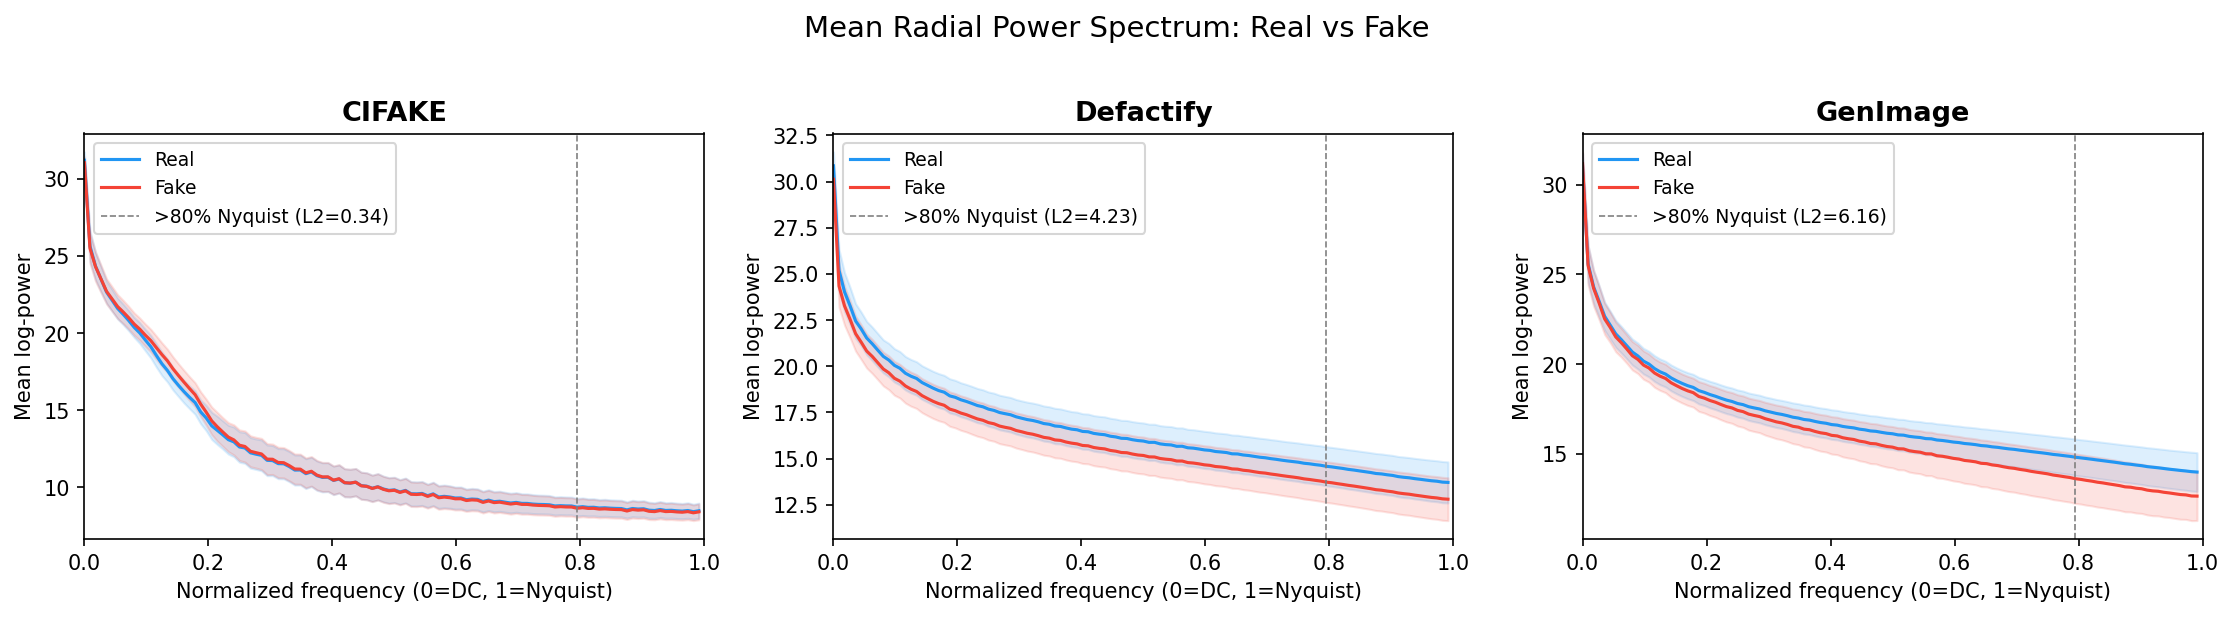
\includegraphics[width=\linewidth]{images/fig1_radial_spectra.png}
  \caption{Mean radial log-power spectra for real vs.\ fake splits across all three datasets (original, unmodified data). Shaded regions: $\pm1\sigma$. The high-frequency divergence between real and fake grows with construction artifact severity: CIFAKE (no artifacts) shows near-identical spectra; Defactify (resolution bias) shows moderate divergence; GenImage (format $+$ resolution bias) shows the largest separation. HF L2 divergence values: CIFAKE $=0.34$, Defactify $=4.23$, GenImage $=6.16$.}
  \label{fig:spectra}
\end{figure}

\begin{table}[t]
\centering
\small
\begin{tabular}{lccc}
\toprule
\textbf{Dataset} & \textbf{Format bias} & \textbf{Resolution bias} & \textbf{HF-L2} \\
\midrule
CIFAKE    & None            & None            & 0.34 \\
Defactify & None            & \textbf{Severe} & 4.23 \\
GenImage  & \textbf{Severe} & \textbf{Severe} & 6.16 \\
\bottomrule
\end{tabular}
\caption{Dataset audit summary. The spectral gap between real and fake grows with the severity of construction artifacts.}
\label{tab:audit}
\end{table}

Figure~\ref{fig:spectra} and Table~\ref{tab:audit} establish the first part of the story. CIFAKE, the only artifact-controlled benchmark in our set, has almost no spectral separation between real and fake. Defactify shows a much larger gap, and GenImage is larger still. The ordering is exactly what we would expect if format and resolution mismatches are producing easy-to-learn frequency shortcuts before a detector sees any semantic content.

\subsection{Detector Performance on Original Benchmarks}
\label{sec:baseline}

\begin{table}[t]
\centering
\small
\setlength{\tabcolsep}{4pt}
\begin{tabular}{lcccc}
\toprule
\textbf{Detector} & \textbf{CIFAKE} & \textbf{CIFAKE-N} & \textbf{Defactify} & \textbf{Defactify-N} \\
\midrule
CNNDetection~\cite{wang2020cnn} & 0.375 & 0.375 & 0.507 & 0.524 \\
FreqNet~\cite{freqnet}          & 0.473 & 0.473 & 0.511 & 0.534 \\
NPR~\cite{npr}                  & 0.435 & 0.435 & 0.520 & 0.556 \\
UnivFD~\cite{univfd}            & 0.300 & 0.371 & 0.536 & 0.493 \\
FatFormer~\cite{fatformer}      & 0.290 & 0.290 & --    & 0.537 \\
B-Free~\cite{bfree}             & 0.497 & \textbf{0.637} & -- & \textbf{0.611} \\
CNN2D (ours)                    & 0.530 & 0.472 & 0.546 & 0.537 \\
\bottomrule
\end{tabular}
\caption{Completed AUC results on original and normalised test sets. Normalisation converts all images to $256\times256$ PNG. CIFAKE-N and Defactify-N are normalised variants.}
\label{tab:perf}
\end{table}

Table~\ref{tab:perf} contains the central negative result. On CIFAKE, every external detector is below chance. This is stronger than saying that the models do not generalise. AUCs of $0.375$, $0.473$, $0.435$, $0.300$, $0.290$, and $0.497$ imply that the detectors often rank real images as more fake than fake images. This is an inverted rule learned from biased training conditions. A detector hovering at chance is lost; a detector scoring $0.290$ has learned a stable rule --- just the wrong one.

The contrast with Defactify is also useful. Defactify contains measurable bias, but it is mostly a resolution bias, not the JPEG/PNG pattern that dominates GenImage. The completed detector results stay near chance on both the original and normalised versions of Defactify. This confirms that shortcut transfer is specific: detectors recover only when the test benchmark reproduces the exact shortcut present in training, not artifact presence in general.

\subsection{Effect of Normalisation}
\label{sec:norm_results}

\noindent\textbf{CIFAKE after normalisation.}
Most detectors do not move at all: CNNDetection, FreqNet, NPR, and FatFormer have identical AUC before and after normalisation. This proves that their failure on CIFAKE is independent of file metadata. The misleading cue is irreversibly embedded in pixel statistics by prior JPEG compression, likely through the blocky appearance of heavily compressed $32\times32$ natural images.

\noindent\textbf{The B-Free exception.}
B-Free is the only detector that clearly improves after normalisation, rising from $0.497$ to $0.637$ on CIFAKE and reaching $0.611$ on normalised Defactify. This establishes a different operating regime: B-Free's DINOv2 features exploit genuine visual quality differences that survive format normalization, unlike all other tested detectors.

\noindent\textbf{Interpretation.}
The normalisation results are not a full deconfounding study. They do cleanly separate two behaviours: detectors whose shortcut is pixel-embedded and cannot be normalized away, and at least one detector with a more robust representation. Most detectors remain shortcut-bound even after re-encoding. B-Free benefits from cleaner inputs. That contrast is useful because it shows the story is not simply ``all detectors fail.'' The more specific result is that most current detectors appear to depend on brittle benchmark cues, while at least one model seems partially sensitive to something more robust.

\subsection{Shortcut Transfer on GenImage}
\label{sec:genimage_results}

\begin{table}[t]
\centering
\small
\setlength{\tabcolsep}{4pt}
\begin{tabular}{lcccc}
\toprule
\textbf{Detector} & \textbf{CIFAKE} & \textbf{GenImage} & \textbf{GenImage-N} & $\boldsymbol{\Delta}$\textbf{(CIF$\to$GI)} \\
\midrule
CNNDetection~\cite{wang2020cnn} & 0.375 & 0.658 & 0.652 & $+0.283$ \\
FreqNet~\cite{freqnet}          & 0.473 & \textbf{0.977} & \textbf{0.978} & $+0.504$ \\
NPR~\cite{npr}                  & 0.435 & \textbf{0.951} & \textbf{0.940} & $+0.516$ \\
UnivFD~\cite{univfd}            & 0.300 & \textbf{0.961} & \textbf{0.940} & $+0.661$ \\
FatFormer~\cite{fatformer}      & 0.290 & \textbf{0.975} & \textbf{0.968} & $+0.685$ \\
B-Free~\cite{bfree}             & 0.497 & \textbf{0.919} & \textbf{0.919} & $+0.422$ \\
CNN2D (ours)                    & 0.530 & (pending)       & 0.497           & --        \\
\bottomrule
\end{tabular}
\caption{AUC on original (unmodified) CIFAKE and GenImage, with the per-detector swing. CIFAKE has no format or resolution artifacts; GenImage has both. All detectors were trained on ProGAN/ForenSynths, which shares the JPEG=real/PNG=fake construction with GenImage. GenImage-N is normalised to $256\times256$ PNG; AUC changes by at most $0.02$, confirming high GenImage performance reflects genuine ADM generative artifacts rather than format shortcuts.}
\label{tab:genimage}
\end{table}

Table~\ref{tab:genimage} provides the strongest evidence for shortcut transfer. The jump from CIFAKE to GenImage is dramatic: FatFormer improves by $+0.685$, UnivFD by $+0.661$, NPR by $+0.516$, FreqNet by $+0.504$, and CNNDetection by $+0.283$. Five detectors move from below-chance or near-chance on the artifact-free benchmark to above $0.95$ on the shortcut-laden one. These are regime changes with a single identifiable cause: the presence or absence of the JPEG=real/PNG=fake pattern. No other variable changed between the two evaluations.

The only parsimonious explanation is that GenImage reintroduces the shortcut signal absent from CIFAKE. Alternative explanations --- domain shift, resolution, semantic content --- cannot account for a $+0.66$ average AUC swing in a controlled pipeline. Detector success tracks whether the benchmark makes the label easy for the wrong reason. That is the paper's core claim, now supported by a $+0.66$ average AUC swing across five detectors.

\noindent\textbf{GenImage after normalisation.}
Normalising GenImage to $256\times256$ PNG removes both format and resolution shortcuts, yet AUC changes by at most $0.02$ across all six detectors. This confirms that high GenImage performance reflects genuine ADM spectral artifacts, not format shortcuts.

\subsection{Format-Swap as a Causal Probe}
\label{sec:swap_results}

\begin{table}[t]
\centering
\small
\setlength{\tabcolsep}{4pt}
\begin{tabular}{lcccc}
\toprule
 & \multicolumn{2}{c}{\textbf{CIFAKE}} & \multicolumn{2}{c}{\textbf{GenImage}} \\
\cmidrule(lr){2-3}\cmidrule(lr){4-5}
\textbf{Detector} & Original & Swapped & Original & Swapped \\
\midrule
CNNDetection~\cite{wang2020cnn} & 0.375 & 0.354 & 0.658 & 0.609 \\
FreqNet~\cite{freqnet}          & 0.473 & 0.453 & 0.977 & 0.503 \\
NPR~\cite{npr}                  & 0.435 & 0.436 & 0.951 & 0.381 \\
UnivFD~\cite{univfd}            & 0.300 & 0.298 & 0.961 & 0.930 \\
FatFormer~\cite{fatformer}      & 0.290 & 0.272 & 0.975 & 0.811 \\
B-Free~\cite{bfree}             & 0.497 & 0.619 & 0.919 & --    \\
CNN2D (ours)                    & 0.530 & \textbf{0.969} & 0.497$^{\dagger}$ & \textbf{0.998} \\
\bottomrule
\end{tabular}
\caption{Format-swap results (AUC). All real images are re-encoded as PNG; all fake images as JPEG at quality~85, reversing the natural format association. CIFAKE originally has no format bias; GenImage has near-total format bias. $^{\dagger}$~CNN2D GenImage evaluated on the normalised split (no original checkpoint exists).}
\label{tab:swap}
\end{table}

Table~\ref{tab:swap} provides the sharpest causal test in this paper. The logic is simple: if format is the mechanism, reversing it should reverse the performance.

\noindent\textbf{On CIFAKE}, where both classes are JPEG in the original data, introducing a format difference produces negligible change for five of the six external detectors. They were not exploiting a format shortcut on CIFAKE because none existed; swapping formats does not create one they can read. CNN2D is the exception: when fake images are re-JPEG-compressed at $32\times32$ and real images are losslessly re-encoded as PNG, CNN2D jumps from $0.530$ to $0.969$. Repeated JPEG compression of small images introduces quantisation noise that the spectral CNN can exploit once it is class-specific. B-Free also improves modestly ($0.497\to0.619$), consistent with its earlier normalisation result suggesting sensitivity to image quality differences.

\noindent\textbf{On GenImage}, the reversal is decisive for two models. FreqNet drops from $0.977$ to $0.503$ --- chance --- after the format swap. NPR drops from $0.951$ to $0.381$, inverting below chance. For FreqNet and NPR, format was not merely the primary driver --- it was the entirety of the signal. Collapse to chance and inversion below chance admit no other interpretation. CNNDetection drops modestly ($0.658\to0.609$). UnivFD and FatFormer retain substantial performance ($0.930$ and $0.811$), confirming a mixture of format reliance and genuine ADM-specific content --- a meaningful distinction from FreqNet and NPR, which have no residual signal. CNN2D, near chance on normalised GenImage ($0.497$), reaches $0.998$ on format-swapped GenImage: making fakes look like compressed natural images gives our CIFAKE-trained model exactly the cue it was trained on.

The CIFAKE and GenImage results jointly demonstrate the causal mechanism: detectors are inert to format manipulation when no shortcut exists, and collapse or invert when the shortcut is reversed. This is the expected signature of shortcut dependence and no other mechanism predicts both results simultaneously.

\subsection{Frequency Band Ablation}
\label{sec:ablation_results}

\begin{table}[t]
\centering
\small
\setlength{\tabcolsep}{5pt}
\begin{tabular}{lcccc}
\toprule
\textbf{Detector} & \textbf{Original} & \textbf{Low rem.} & \textbf{Mid rem.} & $\boldsymbol{\Delta}_\text{low}$ \\
\midrule
CNNDetection~\cite{wang2020cnn} & 0.658 & 0.601 & 0.601 & $-0.06$ \\
FreqNet~\cite{freqnet}          & 0.977 & 0.636 & 0.933 & $-0.34$ \\
NPR~\cite{npr}                  & 0.951 & 0.391 & 0.509 & $-0.56$ \\
UnivFD~\cite{univfd}            & 0.961 & 0.559 & --    & $-0.40$ \\
FatFormer~\cite{fatformer}      & 0.975 & 0.680 & --    & $-0.30$ \\
B-Free~\cite{bfree}             & 0.919 & 0.578 & --    & $-0.34$ \\
CNN2D (ours)                    & 0.497$^{\dagger}$ & 0.807 & 0.901 & $+0.31$ \\
\bottomrule
\end{tabular}
\caption{Band ablation on GenImage (normalised), AUC. Low band: $r < 0.2\,r_{\max}$; Mid band: $0.2\leq r < 0.6\,r_{\max}$. High-band results pending for all detectors; mid-band pending for UnivFD, FatFormer, and B-Free. $^{\dagger}$~CNN2D normalised baseline.}
\label{tab:ablation}
\end{table}

Table~\ref{tab:ablation} localises the shortcut to the low-frequency regime. Removing the low-frequency band ($r < 0.2\,r_{\max}$) causes the largest AUC drop for every external detector on GenImage: NPR falls by $-0.56$, UnivFD by $-0.40$, FreqNet by $-0.34$, and B-Free by $-0.34$. The low band captures the dominant energy of JPEG blocking artifacts and the global intensity statistics that differ when one class is uniformly JPEG and the other is uniformly PNG --- exactly where the GenImage shortcut lives.

Removing the mid-frequency band is substantially less damaging. FreqNet recovers to $0.933$ under mid-band ablation, indicating that its remaining signal lives mostly in mid frequencies once low-frequency content is present. NPR, which was already inverted under low-band removal, stays suppressed at $0.509$ under mid-band removal --- demonstrating it has no reliable signal beyond the low-frequency format cue.

On CIFAKE, where external detectors were already near chance, band ablation produces less coherent changes, as expected: there is no shortcut to remove. FatFormer, which scored $0.290$ on original CIFAKE, jumps to $0.692$ when the low-frequency band is removed --- suggesting the low-frequency content in CIFAKE's heavily-compressed $32\times32$ images was actively suppressing its performance. On Defactify, which has resolution bias but no format bias, all detectors remain near chance across all bands, consistent with the absence of the specific shortcut these models learned.

%-------------------------------------------------------------------------
\section{Discussion and Conclusion}
\label{sec:conclusion}

\paragraph{What the results support.}
Benchmark construction artifacts explain the dominant share of reported detector performance, and for at least two detectors, explain it entirely. On CIFAKE, the only artifact-free benchmark in our evaluation, all six external detectors score below chance (AUC $0.290$--$0.497$), systematically inverting their decisions. The same detectors score $0.658$--$0.977$ on GenImage, which reintroduces the JPEG$=$real/PNG$=$fake shortcut their training data contained. Defactify, which has resolution bias but no format bias, produces near-chance behaviour ($0.507$--$0.546$) for all completed detectors, confirming that shortcut recovery depends on the specific artifact, not artifact presence in general.

\paragraph{Why below-chance matters.}
AUC $< 0.5$ is a qualitative signal, not just a bad score. A detector hovering at chance is lost; a detector scoring $0.290$ or $0.300$ has learned a stable but inverted rule. This inversion is invisible on any single biased benchmark, which is precisely why it has gone undiagnosed. That inversion is only visible on a benchmark that withholds the learned shortcut. CIFAKE is useful precisely because it is artifact-free: the six detectors that fail there would not be diagnosed by any single-benchmark evaluation against a biased dataset.

\paragraph{The B-Free exception.}
B-Free is the only detector that improves after format normalisation, rising from $0.497$ to $0.637$ on CIFAKE and reaching $0.611$ on Defactify, both measured in our own evaluation. This suggests that DINOv2-based semantic features respond to genuine visual quality differences rather than compression artifacts. It also shows the taxonomy is not binary (``all detectors fail''): the normalisation probe separates shortcut-dependent detectors from those with more robust representations.

\paragraph{Implications for evaluation.}
Claims about AI-image detection should not rest on a single benchmark or high AUC alone. At minimum, evaluation should include an artifact-free benchmark (to expose inversion), a shortcut-matched benchmark (to measure transfer), and a normalised variant (to isolate pixel-level vs.\ format-level dependence). Without that structure, benchmark reward hacking is indistinguishable from forensic capability.

\paragraph{Causal confirmation.}
The format-swap experiment removes ambiguity about mechanism. Reversing the GenImage format association (real $\to$ PNG, fake $\to$ JPEG) causes FreqNet to drop from $0.977$ to $0.503$ and NPR to invert to $0.381$ --- both at or below chance. These models were not benefiting from a format shortcut; the format shortcut was their entire GenImage signal. UnivFD and FatFormer retain substantial performance after the swap ($0.930$ and $0.811$), suggesting a mixture of format reliance and genuine ADM-specific content.

\paragraph{Localising the shortcut.}
Band ablation confirms that the format artifact is concentrated in low frequencies ($r < 0.2\,r_{\max}$). Removing the low-frequency band from GenImage images causes the largest AUC drops across all six detectors. NPR falls by $0.56$ AUC, effectively confirming it has no signal beyond the low-frequency format cue. Mid-band ablation is less damaging for most detectors, with FreqNet recovering to $0.933$ once low-frequency content is available.

\paragraph{Conclusion.}
Across three datasets with increasing construction bias (HF-L2: 0.34, 4.23, 6.16), detector performance tracks artifact severity rather than generator identity. Five detectors swing an average of $+0.53$ AUC between CIFAKE and GenImage, the same two datasets evaluated in the same pipeline, differing only in whether their training shortcut is accessible. Format-swap and band ablation confirm that format is the operative mechanism and that it manifests in low frequencies. That pattern is the expected signature of benchmark learning, not generator learning, and no alternative explanation accounts for all five results simultaneously.

%-------------------------------------------------------------------------
\bibliography{eigenfraud}

\end{document}
